\documentclass{article}
\usepackage{amsmath}
\usepackage{amsfonts}
\usepackage{amssymb}
\usepackage{mathrsfs}
\usepackage{dsfont}
\usepackage{cancel}

\usepackage{graphicx}


\setlength\parindent{0pt}

\author{Pranav Tikkawar}
\title{Chapter 2 }

\begin{document}
\maketitle
\section*{2.1 Wave Equation}
$$ u_{tt} = c^2 u_{xx}, x \in \mathds{R} ***$$
\textbf{Theorem 1: d'Alembert}\\
Any solution to *** is of form $$ u(x,t) = f(x + ct) + g(x - ct) $$  where $f$ and $g$ are twice differentiable functions.\\
\textbf{Proof:} Method 1\\
$$ (d_t^2 - c^2 d_x^2 )u  = 0 $$
$$ (d_t - c d_x)(d_t + c d_x)u = 0 $$
Let $ v = (d_t + c d_x)u $\\
Then $ (d_t - c d_x)v = 0 $
This is a transport equation. The general solution is $$ v(x,t) = h(x + ct) $$ for some function $h$.\\
$$ u_t + c u_x  = f(x + ct) $$
Inhomogeneous transport equation.\\
We can use linearity to find the general solution. Since it will be the sum of homogenous plus another function\\
$$ u = u_p + g(x-ct) $$
Where $u_p$ is a particular solution.\\
$$ u_p = h(x + ct) $$
$$h'c + ch' =  f$$ 
$$h' = \frac{f}{2c}$$
$$ u = \frac{1}{2c} \int f(x + ct) dx + g(x - ct)$$***

$$(\partial_t - c \partial_x)(\partial_t + c \partial_x)u = 0 $$
$$ f(x+ct), g(x-ct)$$
Recall that $f(x+ct)$ is a wave traveling left at speed c and $g(x-ct)$ is a wave traveling right at speed c\\
Thus the solution is a wave traveling with speed c in both directions.\\
The wave equation is bidirectional.(unlike the transport equation)\\
\textbf{Remark:} u is a superposition of two waves traveling in opposite directions at fixed speed c.\\
\textbf{Method 2:} \\
Characteristic variable: 
$$ \xi = x + ct, \eta = x - ct $$
Then we can write 
$$ u(x,t) = u(\xi(x,t),\eta(x,t)) $$
$$ \partial_x = \partial_\xi + \partial_\eta $$
$$ \partial_t = c \partial_\eta - c \partial_\xi $$
Factoring gives us 
$$ \partial_t^2 - c^2 \partial_x^2 = (\partial_t -c\partial_x)(\partial_t + c \partial_x) $$
Plugging in we get 
$$ -2c\partial_\eta \cdot 2c \partial_\xi  $$
$$ -4c^2 \partial_\xi \partial_\eta = 0 $$ 
Thus we can differentiate with respect to $\xi$ and $\eta$ to get the general solution.
$$ u_{\xi \eta} = 0 $$
Integrating gives us
$$ u = f(\xi) + g(\eta) $$
\textbf{Theorem 2: (d'Alembert 1747)}
$$\begin{cases}
    u_{tt} = c^2 u_{xx}, t>0, x \in \mathds{R}\\
    u(x,0) = \phi(x), x \in \mathds{R}\\
    u_t(x,0) = \psi(x), x \in \mathds{R}
\end{cases} 
$$
Where $\phi$ is initial displacement and $\psi$ is initial velocity.\\
$$ u(x,t) = \frac{1}{2} \left( \phi(x + ct) + \phi(x - ct) \right) + \frac{1}{2c} \int_{x - ct}^{x + ct} \psi(s) ds $$
\textbf{Proof:} By theorum 1: 
$$ u(x,t) = f(x+ct) + g(x-ct)$$
Find f,g using ICs 
$$ u(x,0) = f(x) + g(x) = \phi(x) $$
$$ u_t(x,t) = cf'(x+ct) - cg'(x-ct) $$
$$ u_t(x,0) = c f'(x) - c g'(x) = \psi(x) $$
$$\begin{cases}
    c f' + cg' = c \phi'\\
    c f' - cg' = \psi
\end{cases}
$$
Adding gives us
$$\begin{cases}
    2cf' = c \phi' + \psi\\
    2cg' = c \phi' - \psi
\end{cases}
$$
$$
\begin{cases}
    f' = \frac{1}{2} \left( \phi' + \frac{\psi}{c} \right)\\
    g' = \frac{1}{2} \left( \phi' - \frac{\psi}{c} \right)
\end{cases}
$$
$$f(s) = \frac{1}{2} \phi(s) + \frac{1}{2c} \int_0^s \psi(y) dy + A$$
$$g(s) = \frac{1}{2} \phi(s) - \frac{1}{2c} \int_0^s \psi(y) dy + B$$
$$
\begin{cases}
    f(0) = \frac{1}{2} \phi(0) + A\\
    g(0) = \frac{1}{2} \phi(0) + B
\end{cases}
$$
$$
f(0) + g(0) = \phi(0) + A + B
$$
$f+g = \phi$ which cancels outs\\
Thus we can set $A + B= 0 $\\
\begin{align*}
    u(x,t) &= f(\xi) + g(\eta)\\
    &= \frac{1}{2}\phi(\xi) + \frac{1}{2c} \int_0^\xi \psi(y) dy + A \\
    &+ \frac{1}{2}\phi(\eta) - \frac{1}{2c} \int_0^\eta \psi(y) dy + B
\end{align*}
\begin{align*}
    u(x,t) &= f(\xi) + g(\eta)\\
    &= \frac{1}{2}\phi(\xi) + \frac{1}{2c} \int_0^\xi \psi(y) dy  \\
    &+ \frac{1}{2}\phi(\eta) - \frac{1}{2c} \int_0^\eta \psi(y) dy\\
    &= \frac{\phi(\xi) + \psi(\eta)}{2} + \frac{1}{2c} \left( \int_0^\xi \psi(y) dy - \int_0^\eta \psi(y) dy \right)\\
    &= \frac{\phi(\xi) + \psi(\eta)}{2} + \frac{1}{2c} \int_{\eta}^{\xi} \psi(y) dy
\end{align*}
2 families of characteristics lines:\\
$$ x \pm ct = constant$$
On one of these lines they are constant.\\
\textbf{Example 1: }\\
$\psi(x) = 0$\\
$$ u(x,t) = \frac{1}{2} \left( \phi(x + ct) + \phi(x - ct) \right)$$
Initial displacement $\phi$ splits into two parts. Each with half the amplitude. and one is opposite direction from the other\\
\textbf{Example 2: }\\
$\psi(x) = 0$\\
Interaction of "pulse".\\
They constructively interfere and they keep their shape.\\
\textbf{Example 3: }\\
$\phi(x) = 0$\\
$$ u(x,t) = \frac{1}{2c} \int_{x - ct}^{x + ct} \psi(y) dy$$
If x is too large of magnititue it will be zero.\\
As we increase t, the integral will increase.\\
For largers t, I have more choses of x that make u nonzero.\\
\textbf{Example 4: }\\
$\psi(x) = 0, \phi(s) = sin(s)$
$$ u(x,t) = \frac{1}{2} \left( sin(x + ct) + sin(x - ct) \right)$$
$$ u(x,t) = sin(x) cos(ct)$$
This is a standing wave! 
\textbf{Remark 1:}\\
If $\psi = 0$ and $\phi$ is localized then the right and left moving waves will (in the long run) always separate.\\
If $\phi$ is not localized then then they don't separate
\textbf{Remark 2:} $\phi = 0 $ and $\psi$ is localized, fix $x_0$ then $u(x_0,t) = 0 $ for all $t >t_0$.\\
The intial disturbance is felt at $x_0$ and then the affect will be gone
\section*{2.2 Causality and Energy }
$$\begin{cases}
    u_{tt} = c^2 u_{xx} \\
    u(x,0) = \phi(x)\\
    u_t(x,0) = \psi(x)
\end{cases}
$$
D'Alembert solution:
$$ u(x,t) = \frac{1}{2} \left( \phi(x + ct) + \phi(x - ct) \right) + \frac{1}{2c} \int_{x - ct}^{x + ct} \psi(s) ds $$
\textbf{Lemma: }
If $\phi$ and $\psi$ are compactly supported in $[a,b]$, (this means outside the interval they are zero) then $u(x,t) = 0$ outside of $R$ where R is the "domain of influence of the interval $[a,b]$\\
The boundary lines are $x - ct =b$ and $x + ct = a$\\
This is like an open cone.\\
$$ R = \text{ regieon where distubances are felt}$$
\textbf{Proof:}\\
By assumption $\phi(s)$ and $\psi(s)$ are zero for $s < a $\\
Thus the outside area is $x + ct < a$\\
Also $x - ct \leq x+ct < a$\\
In that region $u(x,t) = 0$\\
Similarly we can do this for the region $x - ct > b$\\
Thus we can conclude that $u(x,t) = 0$ outside of the region $R$. Due to the fact that both $\phi =0$ and the integral $\int_{x-ct}^{x+ct} \psi(s) ds = 0$ \\

In the limiting case. This is a "light cone"\\
This is where we have $x_0$ being the point of disturbance.\\
The region of influence is the area where the disturbance is felt.\\ 
$$ x +ct = x_0, x - ct = x_0$$
$$ x \pm ct = x_0$$

$ \phi(x_0)$ and $\psi(x_0)$ affect the values of $u(x,t)$ if $x \pm ct = x_0$ or $x_0 \in [x - ct, x + ct]$\\

\textbf{Reverse Questions:}\\
Fix value of u and see what initial conditions affect this.\\
We need initial values at $x_0 \pm ct_0$ and in $[x_0 - ct_0, x_0 + ct_0]$\\
This is like a triangle\\
This is called the interval/region of dependance of the point $x_0$.\\
\textbf{Remark: }\\
$$u(x_0,t_0) = \frac{1}{2} \left( \phi(a) + \phi(b) \right) + \frac{1}{2c} \int_{a}^{b} \psi(s) ds$$
$$b-a = 2ct_0$$
$$ u(x_0,t_0) = \frac{1}{2} \left( \phi(a) + \phi(b) \right) + t_0 \cdot \frac{1}{b-a} \int_{a}^{b} \psi(s) ds$$
Note that the first term is average displacement and the second term is average velocity.\\
\textbf{Example: }\\
$$\psi = 0, \phi = \begin{cases}
    1, & x \in [0,1]\\
    0, & \text{otherwise}
\end{cases}
$$
say $c =1 $\\
Now: add image of the region of influence.\\
\begin{center}
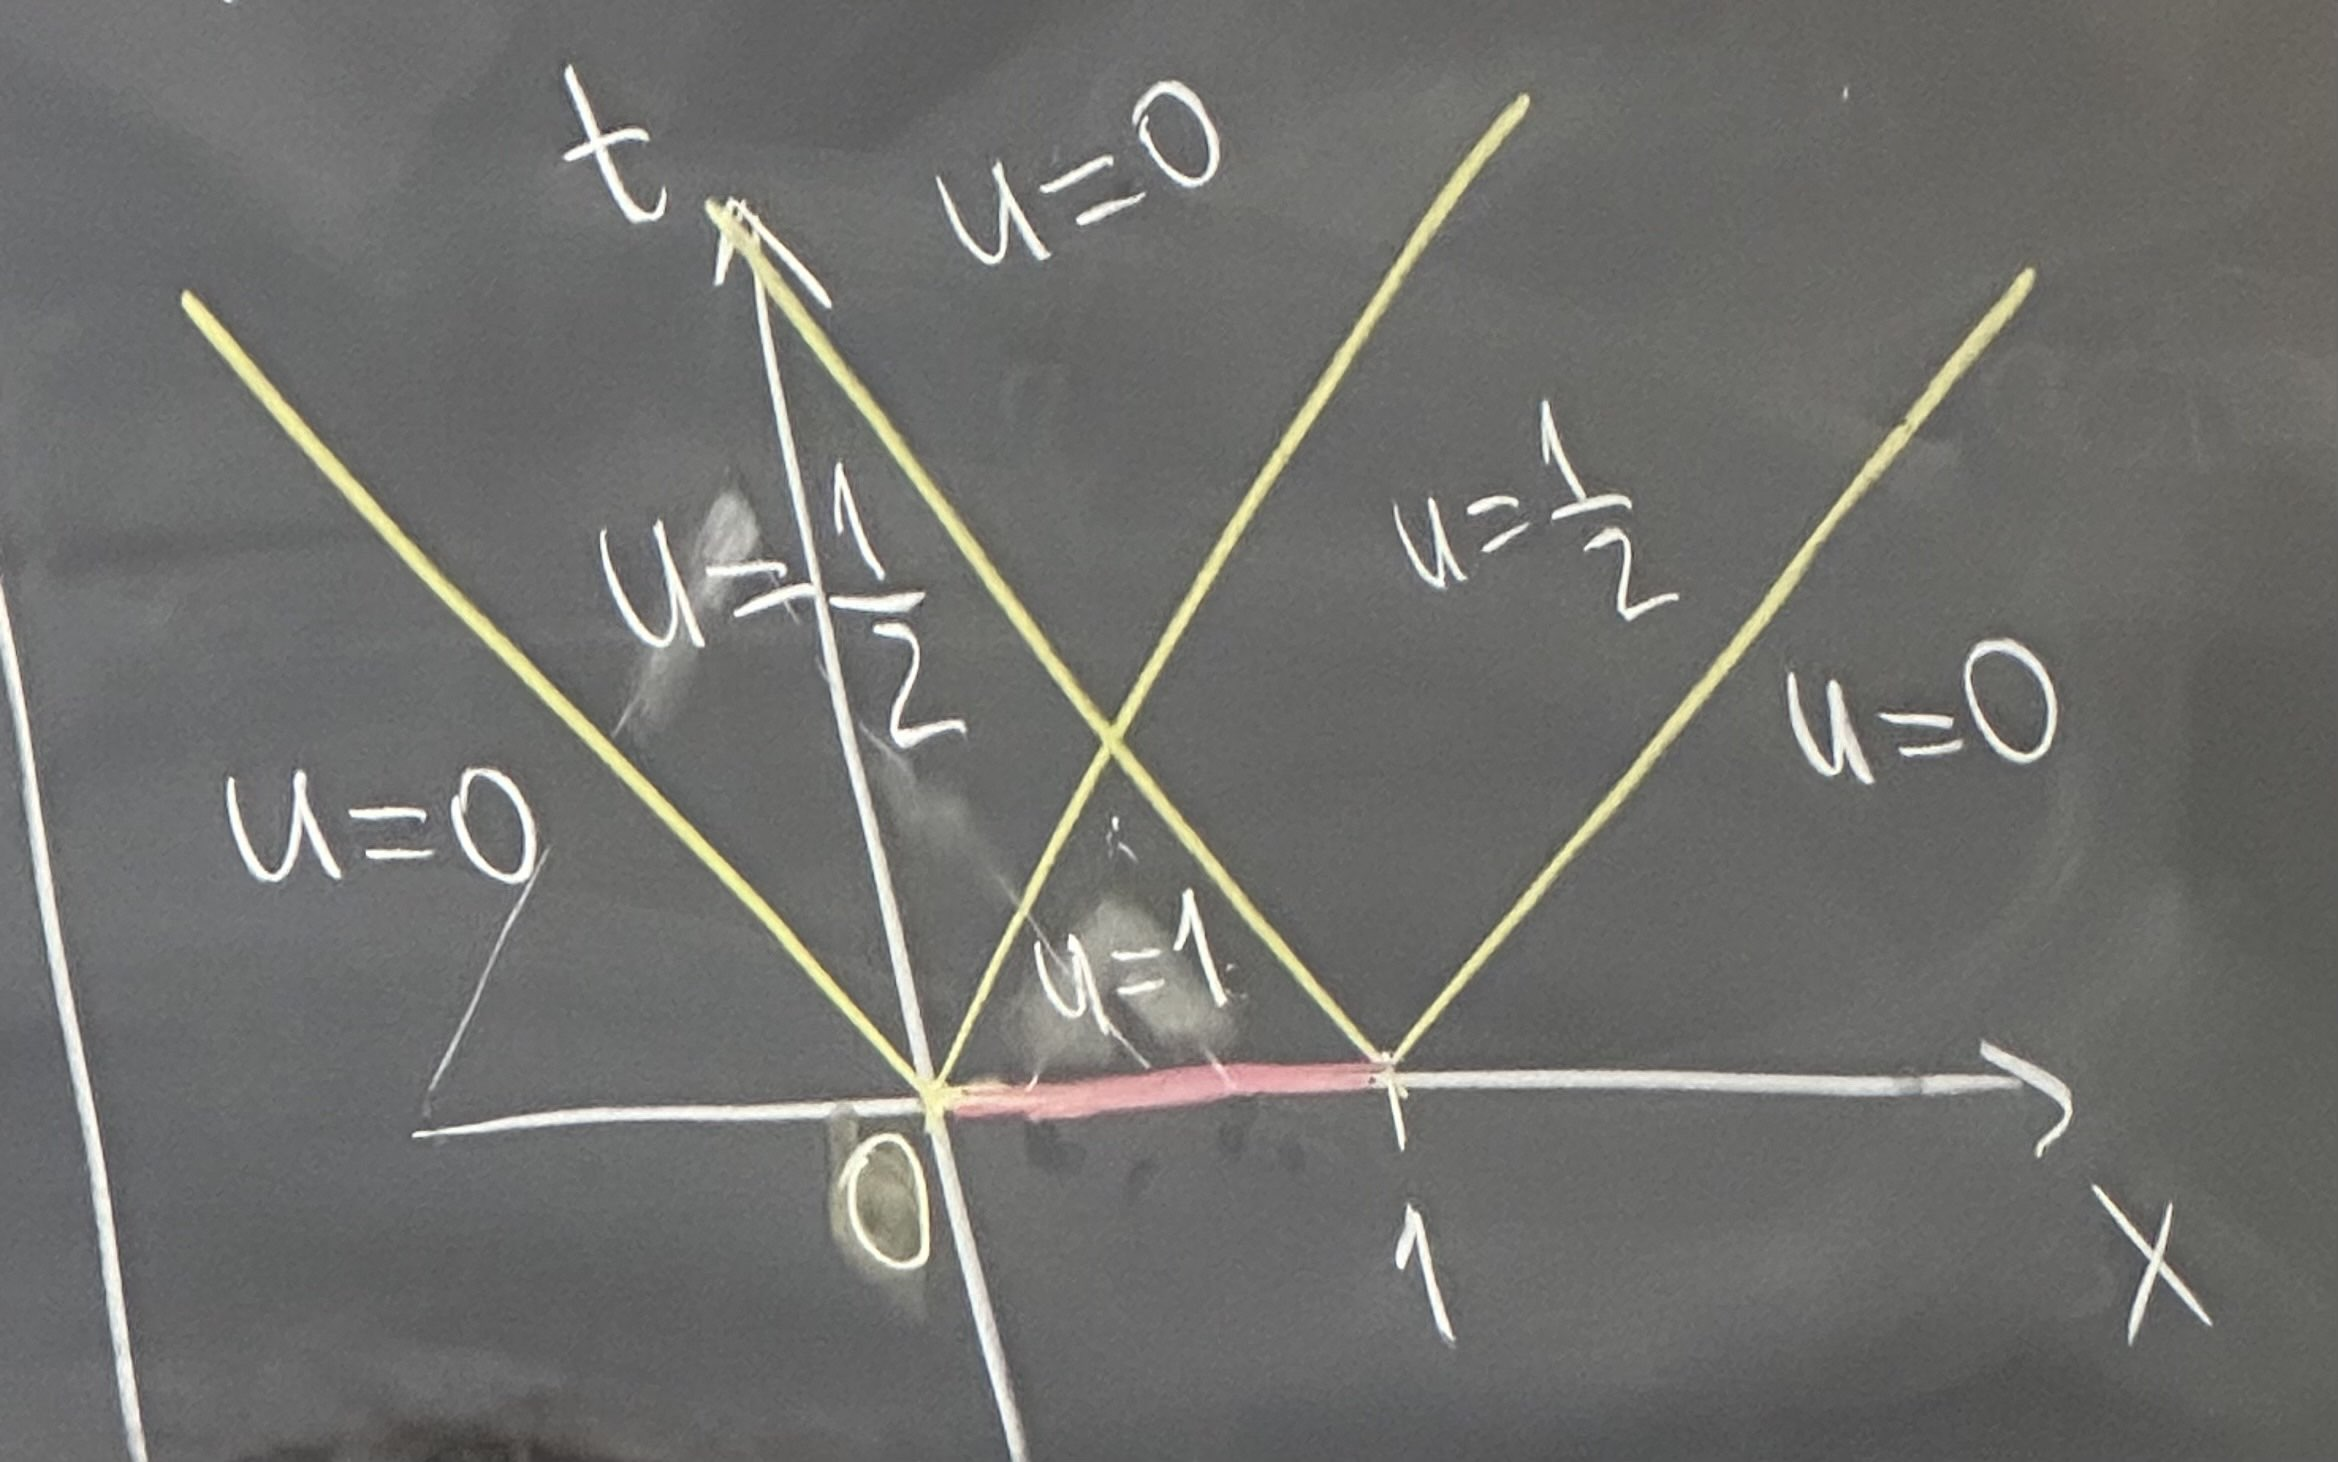
\includegraphics[width=0.5\textwidth]{IMGs/PDEs_Triangle.jpg}
\end{center}
We can view this as two Vs that intersect at a point and then separate.\\
Outside the two Vs it is 0, inside both it is 1, inside one it is 1/2\\
And if it is in the middle it is also 0\\
\textbf{Finite speed of propagation:}\\
Localized initial data ie compactly supported. (0 outside some interval)\\
This implies that $u(x,t)$ is also localize for any $t>0$.\\
If $\phi, \psi$ are supported in $[a,b]$ then $u(x,t)$ is supported in $[a-ct,b+ct]$\\
when you are at position $x$ you would feel the disturbance at time $t \geq \frac{x-b}{c}$ or distance from $x$ to the interval

\textbf{Remark:} \\
The wave equation has no smoothing effect.\\
Singularity and discontinuities remain \\
Non-smooth initial data does not become smooth at any time.\\
Say $\phi$ has a discontinuity/ singularuty at $x_0$, then $u(x,t)$ is singular whenever $x \pm ct = x_0$\\
Singularity propogrates along characteristics.\\

\textbf{Causality: }\\
Causality means the effect comes after the cause.\\
Cause = distubance at $x_0$\\
Effect = disturbance at other points\\
Since there is a finite speed of propagation, the disturbance at $x_0$ can only affect points in the region of influence.\\

\textbf{Huygen's Principle:} \\
The disturbance in $[a,b]$ reaches $x_1$ at time $t_1$ and then it remains in the region of influence for all $t > t_1$.\\
If $\psi = 0$ region of influence of $[a,b]$ is just the effect is felt only at time $t_1$ and no lingering effects. In other words, just feel once then gone.\\
\textbf{Kirkchoff's formula}\\
In 3d the solution to the wave equation is given by Kirkchoff's formula.\\
it only uses $\phi$ and $\psi$ on the boundary of the region of influence.\\
this is true for $n \geq 3$ and odd dimensions.\\
So in 2D this is not true! 



\end{document}